\documentclass[14pt,a4paper]{extarticle}
% =============================================================
% preamble.tex — оформление отчётов по СТП БГУИР 01-2024
% =============================================================

% Шрифты: под pdflatex — Times через tempora + T2A,
% под xelatex/tectonic — системный Times New Roman (запасной вариант STIX Two Text)
\usepackage{iftex}
\ifPDFTeX
  \usepackage[utf8]{inputenc}
  \usepackage[T2A]{fontenc}
  \usepackage{tempora}
\else
  \usepackage{fontspec}
  \IfFontExistsTF{Times New Roman}
    {\setmainfont{Times New Roman}}
    {\setmainfont{STIX Two Text}}
  \IfFontExistsTF{DejaVu Sans Mono}
    {\setmonofont{DejaVu Sans Mono}[Scale=0.82]}
    {\setmonofont{DejaVuSansMono}[Extension=.ttf, BoldFont=*-Bold,
                                  ItalicFont=*-Oblique, Scale=0.82]}
\fi
\usepackage[russian]{babel}

% Поля: слева 30 мм, справа 15 мм, сверху и снизу 20 мм
\usepackage{geometry}
\geometry{left=30mm, right=15mm, top=20mm, bottom=20mm}

\usepackage{setspace}
\singlespacing

\pretolerance=1000
\tolerance=2000
\emergencystretch=3em

\usepackage{indentfirst}
\setlength{\parindent}{1.25cm}

% Номер страницы — снизу справа
\usepackage{fancyhdr}
\pagestyle{fancy}
\fancyhf{}
\fancyfoot[R]{\thepage}
\renewcommand{\headrulewidth}{0pt}
\fancypagestyle{plain}{%
  \fancyhf{}%
  \fancyfoot[R]{\thepage}%
  \renewcommand{\headrulewidth}{0pt}%
}

\usepackage{amsmath,amssymb}
\usepackage{graphicx}
\usepackage{float}
\usepackage{booktabs}
\usepackage{tabularx}
\usepackage{multirow}
\usepackage{longtable}
\usepackage{array}

\usepackage{caption}
\captionsetup[figure]{labelsep=endash, justification=centering,
                      font={normalsize}, name=Рисунок}
\captionsetup[table]{labelsep=endash, justification=raggedright,
                     singlelinecheck=false, font={normalsize}, name=Таблица}

\usepackage{titlesec}
\titleformat{\section}
  {\normalfont\fontsize{14}{18}\selectfont\bfseries}
  {\thesection}{0.5em}{\MakeUppercase}
\titlespacing*{\section}{1.25cm}{0pt}{14pt}
% Разрыв страницы до заголовка, чтобы номер в содержании совпадал со страницей раздела
\newcommand{\sectionbreak}{\clearpage}
\titleformat{\subsection}
  {\normalfont\fontsize{14}{18}\selectfont\bfseries}
  {\thesubsection}{0.5em}{}
\titlespacing*{\subsection}{1.25cm}{14pt}{14pt}
\titleformat{\subsubsection}
  {\normalfont\fontsize{14}{18}\selectfont\bfseries}
  {\thesubsubsection}{0.5em}{}
\titlespacing*{\subsubsection}{1.25cm}{14pt}{14pt}

\newcommand{\sectioncenter}[1]{%
  \newpage
  \phantomsection
  \addcontentsline{toc}{section}{#1}
  \begin{center}\textbf{\MakeUppercase{#1}}\end{center}
  \vspace{14pt}
}

\usepackage{tocloft}
\renewcommand{\cftsecfont}{\normalfont}
\renewcommand{\cftsecpagefont}{\normalfont}
\renewcommand{\cftsubsecfont}{\normalfont}
\renewcommand{\cftsubsecpagefont}{\normalfont}
\renewcommand{\cftsecleader}{\cftdotfill{\cftdotsep}}
\renewcommand{\cftdotsep}{1}
% babel переопределяет заголовки после преамбулы, поэтому правим через \addto
\addto\captionsrussian{\renewcommand{\contentsname}{\hfill\textbf{СОДЕРЖАНИЕ}\hfill}}
\renewcommand{\cftaftertoctitle}{\hfill}

\usepackage{enumitem}
\setlist[itemize]{noitemsep, topsep=0pt, leftmargin=1.25cm, label=--}
\setlist[enumerate]{noitemsep, topsep=0pt, leftmargin=1.25cm}

% Листинги кода и вывода программы
\usepackage{listings}
\usepackage{fancyvrb}
\lstset{
  basicstyle=\ttfamily\footnotesize,
  frame=single,
  breaklines=true,
  showstringspaces=false,
  inputencoding=utf8,
  extendedchars=true,
  columns=fullflexible,
  keepspaces=true,
  captionpos=t
}
\ifPDFTeX
\lstset{
  literate={а}{{\cyra}}1 {б}{{\cyrb}}1 {в}{{\cyrv}}1 {г}{{\cyrg}}1
           {д}{{\cyrd}}1 {е}{{\cyre}}1 {ж}{{\cyrzh}}1 {з}{{\cyrz}}1
           {и}{{\cyri}}1 {й}{{\cyrishrt}}1 {к}{{\cyrk}}1 {л}{{\cyrl}}1
           {м}{{\cyrm}}1 {н}{{\cyrn}}1 {о}{{\cyro}}1 {п}{{\cyrp}}1
           {р}{{\cyrr}}1 {с}{{\cyrs}}1 {т}{{\cyrt}}1 {у}{{\cyru}}1
           {ф}{{\cyrf}}1 {х}{{\cyrh}}1 {ц}{{\cyrc}}1 {ч}{{\cyrch}}1
           {ш}{{\cyrsh}}1 {щ}{{\cyrshch}}1 {ъ}{{\cyrhrdsn}}1
           {ы}{{\cyrery}}1 {ь}{{\cyrsftsn}}1 {э}{{\cyrerev}}1
           {ю}{{\cyryu}}1 {я}{{\cyrya}}1 {ё}{{\cyryo}}1
           {А}{{\CYRA}}1 {Б}{{\CYRB}}1 {В}{{\CYRV}}1 {Г}{{\CYRG}}1
           {Д}{{\CYRD}}1 {Е}{{\CYRE}}1 {Ж}{{\CYRZH}}1 {З}{{\CYRZ}}1
           {И}{{\CYRI}}1 {Й}{{\CYRISHRT}}1 {К}{{\CYRK}}1 {Л}{{\CYRL}}1
           {М}{{\CYRM}}1 {Н}{{\CYRN}}1 {О}{{\CYRO}}1 {П}{{\CYRP}}1
           {Р}{{\CYRR}}1 {С}{{\CYRS}}1 {Т}{{\CYRT}}1 {У}{{\CYRU}}1
           {Ф}{{\CYRF}}1 {Х}{{\CYRH}}1 {Ц}{{\CYRC}}1 {Ч}{{\CYRCH}}1
           {Ш}{{\CYRSH}}1 {Щ}{{\CYRSHCH}}1 {Ъ}{{\CYRHRDSN}}1
           {Ы}{{\CYRERY}}1 {Ь}{{\CYRSFTSN}}1 {Э}{{\CYREREV}}1
           {Ю}{{\CYRYU}}1 {Я}{{\CYRYA}}1 {Ё}{{\CYRYO}}1
           {—}{{---}}1 {–}{{--}}1 {…}{{\ldots}}1
}
\fi

% Подписи листингов — в том же стиле, что таблицы: «Листинг X.Y — Название»
\captionsetup[lstlisting]{labelsep=endash, justification=raggedright,
                          singlelinecheck=false, font={normalsize}}
\renewcommand{\lstlistingname}{Листинг}
\AtBeginDocument{\numberwithin{lstlisting}{section}}

\lstdefinestyle{python}{language=Python, keywordstyle=\bfseries}
\lstdefinestyle{shell}{language=bash, keywordstyle=\mdseries}
\lstdefinestyle{plain}{language={}, basicstyle=\ttfamily\scriptsize}

% Абзац после листинга должен сохранять отступ 1,25 см (СТП 2.1.1)
\makeatletter
\AtBeginDocument{\let\@endpetrue\@endpefalse}
\makeatother

% Подпись к блоку verbatim: \captionof вне плавающего окружения
% глобально обнуляет \parindent, поэтому отступ восстанавливается вручную
\newcommand{\listingcaption}[2]{%
  \captionof{lstlisting}{#1}\label{#2}%
  \setlength{\parindent}{1.25cm}%
}

\usepackage{hyperref}
\hypersetup{colorlinks=true, linkcolor=black, urlcolor=blue, citecolor=black}

\numberwithin{figure}{section}
\numberwithin{table}{section}
\numberwithin{equation}{section}

% Титульный лист отчёта по лабораторной работе
\newcommand{\makelabtitle}[2]{%
  \begin{titlepage}
  \thispagestyle{empty}
  \begin{center}

  МИНИСТЕРСТВО ОБРАЗОВАНИЯ РЕСПУБЛИКИ БЕЛАРУСЬ

  \vspace{0.5em}
  Учреждение образования

  \vspace{0.5em}
  \textbf{<<Белорусский государственный университет информатики и радиоэлектроники>>}

  \vspace{2em}
  Факультет компьютерных систем и сетей

  \vspace{0.5em}
  Кафедра программного обеспечения информационных технологий
  \end{center}

  \vspace{3em}
  \begin{center}
  \textbf{ОТЧЕТ}

  \vspace{0.5em}
  по лабораторной работе №#1

  \vspace{0.5em}
  по дисциплине

  \vspace{0.5em}
  <<Технологии компонентного программирования>>

  \vspace{0.5em}
  <<#2>>
  \end{center}

  \vspace{5em}
  \begin{flushright}
  \begin{minipage}{0.5\textwidth}
  \textbf{Выполнил:}\\
  Лебедевич Артем Владимирович\\
  магистрант группы 556301

  \vspace{0.6em}
  \textbf{Преподаватель:}\\
  Герман Олег Витольдович\\
  кандидат технических наук\\
  доцент кафедры ИТАС
  \end{minipage}
  \end{flushright}

  \vfill
  \begin{center}Минск, 2026~г.\end{center}
  \end{titlepage}
}


\newcolumntype{L}{>{\raggedright\arraybackslash}X}

\begin{document}

\makelabtitle{4}{Jython: взаимодействие Java и Python}

\tableofcontents

\section{Цель работы}

Изучить взаимодействие языков Java и Python с помощью Jython. Выполнить примеры из
методических материалов и создать приложение Jython с визуальным классом Java: окном
\texttt{JFrame}, меню которого загружает две разные картинки и рисует синусоиду на
холсте.

\section{Теоретические сведения}

\subsection{Jython}

Jython --- реализация языка Python (версии 2.7) для виртуальной машины Java. Программа
на Jython компилируется в байт-код JVM, поэтому может импортировать классы Java как
обычные модули Python, вызывать их методы, перехватывать исключения Java и наследовать
от классов Java. Обратное направление --- запуск кода Python из программы на Java ---
выполняется вызовом библиотеки. Основные понятия приведены в таблице~\ref{tab:terms}.

\begin{table}[H]
\caption{Основные понятия}
\label{tab:terms}
\centering
\begin{tabularx}{\textwidth}{lL}
\toprule
Понятие & Смысл \\
\midrule
\texttt{jython-standalone.jar} & интерпретатор и стандартная библиотека в одном файле:
\texttt{java -jar jython-standalone-2.7.3.jar script.py} \\
\texttt{from java.io import File} & класс Java импортируется как имя Python \\
\texttt{class MyClass(Object)} & класс Python, наследующий класс Java; его экземпляры ---
объекты Java \\
\texttt{sys.path.append("x.jar")} & добавляет jar-файл в путь импорта \\
\texttt{PythonInterpreter} & класс Java, выполняющий код Python внутри программы на
Java \\
Swing & библиотека графического интерфейса Java: \texttt{JFrame},
\texttt{JMenuBar}, \texttt{JPanel}, \texttt{paintComponent} \\
\bottomrule
\end{tabularx}
\end{table}

\subsection{Установка}

Jython распространяется в виде jar-файла. В работе использован
\texttt{jython-standalone-2.7.3.jar} с Maven Central; контрольная сумма SHA-1
проверяется сравнением с файлом \texttt{.sha1}, который публикует Maven. Для запуска
нужна JDK; использован Temurin 17. Скрипт \texttt{scripts/fetch\_runtimes.py} скачивает
jar в каталог \texttt{tools/}, а модуль \texttt{lab4/runtime.py} находит Java и запускает
сценарии.

\subsection{Различия при работе с JDK 17}

Методичка рассчитана на Java 8. С JDK 17 обнаружились следующие отличия.

\begin{itemize}
\item Инструкции \texttt{import javax.swing as swing} и \texttt{import java.awt as awt}
завершаются ошибкой \texttt{No module named swing}, хотя
\texttt{from javax.swing import JFrame} работает. Начиная с Java 9 классы находятся в
модулях, и сканер пакетов Jython их не перечисляет. Модуль \texttt{jcompat.py}
регистрирует нужные пакеты вызовом \texttt{sys.add\_package}, после чего импорты из
методички работают.
\item Защищённый метод родительского класса вызывается как
\texttt{self.super\_\_paintComponent(g)}, а не \texttt{JPanel.paintComponent(self, g)}.
\item Jython --- это Python 2.7: для функции \texttt{print} нужен
\texttt{from \_\_future\_\_ import print\_function}, а строки с символом $\pi$ задаются
литералами \texttt{u""} (запуск с \texttt{-Dfile.encoding=UTF-8}).
\item Окно \texttt{JFrame} нельзя создать в режиме без экрана
(\texttt{java.awt.headless=true}), поэтому автоматически проверяемая часть выполнена на
\texttt{JPanel} и \texttt{JRootPane}.
\end{itemize}

\section{Реализация}

\subsection{Структура программы}

\listingcaption{Структура лабораторной работы}{lst:tree}
\begin{Verbatim}[fontsize=\scriptsize, frame=single, samepage=true]
lab4/jython/java_version.py  System.getProperty, currentTimeMillis
lab4/jython/hello_world.py   sys.stdout.write и print
lab4/jython/files_demo.py    File, FileWriter, IOException
lab4/jython/my_class.py      класс Python на основе java.lang.Object
lab4/jython/greet_frame.py   JFrame с кнопками Greet и Clear
lab4/jython/image_viewer.py  показ JPEG в компоненте Swing
lab4/jython/array_list.py    коллекция Java в цикле Python
lab4/jython/draw_image.py    рисование в BufferedImage
lab4/jython/call_java_class.py, jy10.py, music_player.py, jcompat.py
lab4/jython/menu_app.py      задание: меню, две картинки, синусоида
lab4/java/com/MyClass.java   класс Java из jar-файла
lab4/java/JythonHelloWorld.java  Java запускает Python
lab4/runtime.py              поиск Java и Jython, запуск сценариев
lab4/cases.py                проверяемые сценарии
lab4/runner.py, lab4/gui.py  вывод в консоль и окно
assets/lab4/                 две картинки: JPEG и PNG
\end{Verbatim}

\subsection{Примеры из методических материалов}

Все примеры выполнены. Первый пример (листинг~\ref{lst:first}) показывает, что класс
Java \texttt{System} используется как модуль Python; следующий создаёт файл средствами
\texttt{java.io} и перехватывает исключение Java \texttt{IOException}; класс
\texttt{MyClass} (листинг~\ref{lst:class}) наследует \texttt{java.lang.Object}, поэтому
его экземпляр является объектом Java: для него работают \texttt{hashCode},
\texttt{getClass} и проверка \texttt{isinstance}.

\begin{lstlisting}[style=python, caption={Класс Java из Python}, label={lst:first}]
from java.lang import System  # Java import

print('Running on Java version: ' + System.getProperty('java.version'))
print('Unix time from Java: ' + str(System.currentTimeMillis()))
\end{lstlisting}

\begin{lstlisting}[style=python, caption={Класс Python, наследующий класс Java}, label={lst:class}]
from java.lang import Object

class MyClass(Object):
    def __init__(self):
        Object.__init__(self)
        self.message = "Hello, world! Form Class"

    def printMessage(self):
        print(self.message)
\end{lstlisting}

Примеры из лекции показывают взаимодействие в обе стороны. Класс
\texttt{com.MyClass} на Java компилируется и упаковывается в jar-файл, после чего
подключается из Jython; программа \texttt{JythonHelloWorld.java}, наоборот, запускает
интерпретатор внутри Java (листинг~\ref{lst:embed}).

\begin{lstlisting}[style=plain, caption={Java запускает Python}, label={lst:embed}]
try (PythonInterpreter python = new PythonInterpreter()) {
    python.exec("print('Hello Python World!')");
    python.exec("from jy10 import greet\ngreet('John')");
    python.set("n", 10);
    python.exec("result = n ** 2");
    System.out.println(python.get("result", Integer.class));
}
\end{lstlisting}

\subsection{Приложение с меню}

Окно собрано из трёх частей: строка меню \texttt{File / Draw / Help}, холст и строка
состояния. Меню \texttt{Draw} содержит пункты \texttt{Picture 1 (JPEG)},
\texttt{Picture 2 (PNG)}, \texttt{Sine wave} и \texttt{Clear} с комбинациями клавиш
\texttt{Cmd+1\ldots 0} (на других системах \texttt{Ctrl}).

Холст --- класс \texttt{Canvas}, наследующий \texttt{JPanel}; его метод
\texttt{paintComponent} написан на Python (листинг~\ref{lst:canvas}). Картинка читается
средствами Java (\texttt{ImageIO.read} понимает и JPEG, и PNG), масштабируется по
размеру холста с сохранением пропорций и центрируется. Синусоида рисуется линией
\texttt{Path2D} из одного отрезка на каждый столбец пикселей; подписаны оси, деления
сетки через $\pi/2$ и метки $0,\pi,2\pi,\dots,4\pi$.

\begin{lstlisting}[style=python, caption={Холст: метод paintComponent}, label={lst:canvas}]
class Canvas(JPanel):
    def paintComponent(self, g):
        self.super__paintComponent(g)  # let Swing paint the background first
        g.setRenderingHint(RenderingHints.KEY_ANTIALIASING, RenderingHints.VALUE_ANTIALIAS_ON)
        width, height = self.getWidth(), self.getHeight()
        if self.mode == "picture":
            self.draw_picture(g, width, height)
        elif self.mode == "sine":
            self.draw_sine(g, width, height)

    def draw_sine(self, g, width, height):
        left, top, w, h = self.sine_frame(width, height)
        x_max = 2 * math.pi * self.PERIODS
        path = Path2D.Double()
        for i in range(w + 1):
            x = x_max * i / float(w)
            if i == 0:
                path.moveTo(px(x), py(math.sin(x)))
            else:
                path.lineTo(px(x), py(math.sin(x)))
        g.setColor(BLUE)
        g.draw(path)
\end{lstlisting}

События всех пунктов меню принимает один объект \texttt{Controller}, который
реализует интерфейс \texttt{ActionListener} и выбирает действие по строке команды
пункта (листинг~\ref{lst:controller}).

\begin{lstlisting}[style=python, caption={Обработка выбора пункта меню}, label={lst:controller}]
class Controller(ActionListener):
    def actionPerformed(self, event):
        command = event.getActionCommand()
        if command in PICTURES:
            self.canvas.show_picture(PICTURES[command])
        elif command == "sine":
            self.canvas.show_sine()
        elif command == "clear":
            self.canvas.clear()
\end{lstlisting}

\subsection{Проверка без экрана}

Строка меню, холст и строка состояния устанавливаются в \texttt{JRootPane}
(листинг~\ref{lst:install}). Такой объект принадлежит каждому \texttt{JFrame}, но
существует и без окна. Благодаря этому режим \texttt{-{}-snapshot} рисует содержимое
окна в файл PNG на машине без экрана, а тесты проверяют пиксели. Режим
\texttt{-{}-popup Draw} дорисовывает в снимок раскрытое меню.

\begin{lstlisting}[style=python, caption={Сборка окна}, label={lst:install}]
def install(root, controller, canvas, status):
    root.setJMenuBar(build_menu_bar(controller))
    root.getContentPane().add(canvas, BorderLayout.CENTER)
    root.getContentPane().add(status, BorderLayout.SOUTH)

class MenuFrame(JFrame):
    def __init__(self, visible=True):
        JFrame.__init__(self, TITLE)
        self.canvas = Canvas()
        self.status = make_status()
        self.controller = Controller(self.canvas, self.status, self)
        install(self.getRootPane(), self.controller, self.canvas, self.status)
        self.setDefaultCloseOperation(JFrame.EXIT_ON_CLOSE)
        self.pack()
        self.setVisible(visible)
\end{lstlisting}

\subsection{Окно проверки}

Окно \texttt{python main.py -{}-lab 4 -{}-gui} написано на wxPython: три кнопки слева
показывают снимок содержимого окна для выбранного вида, три кнопки справа запускают
настоящие окна Swing отдельными процессами JVM, справа расположен список из четырнадцати
сценариев.

\section{Результаты работы программы}

На рисунке~\ref{fig:window} показано окно проверки после выполнения всех сценариев
(14 из 14); на снимке раскрыто меню \texttt{Draw}.

\begin{figure}[H]
\centering
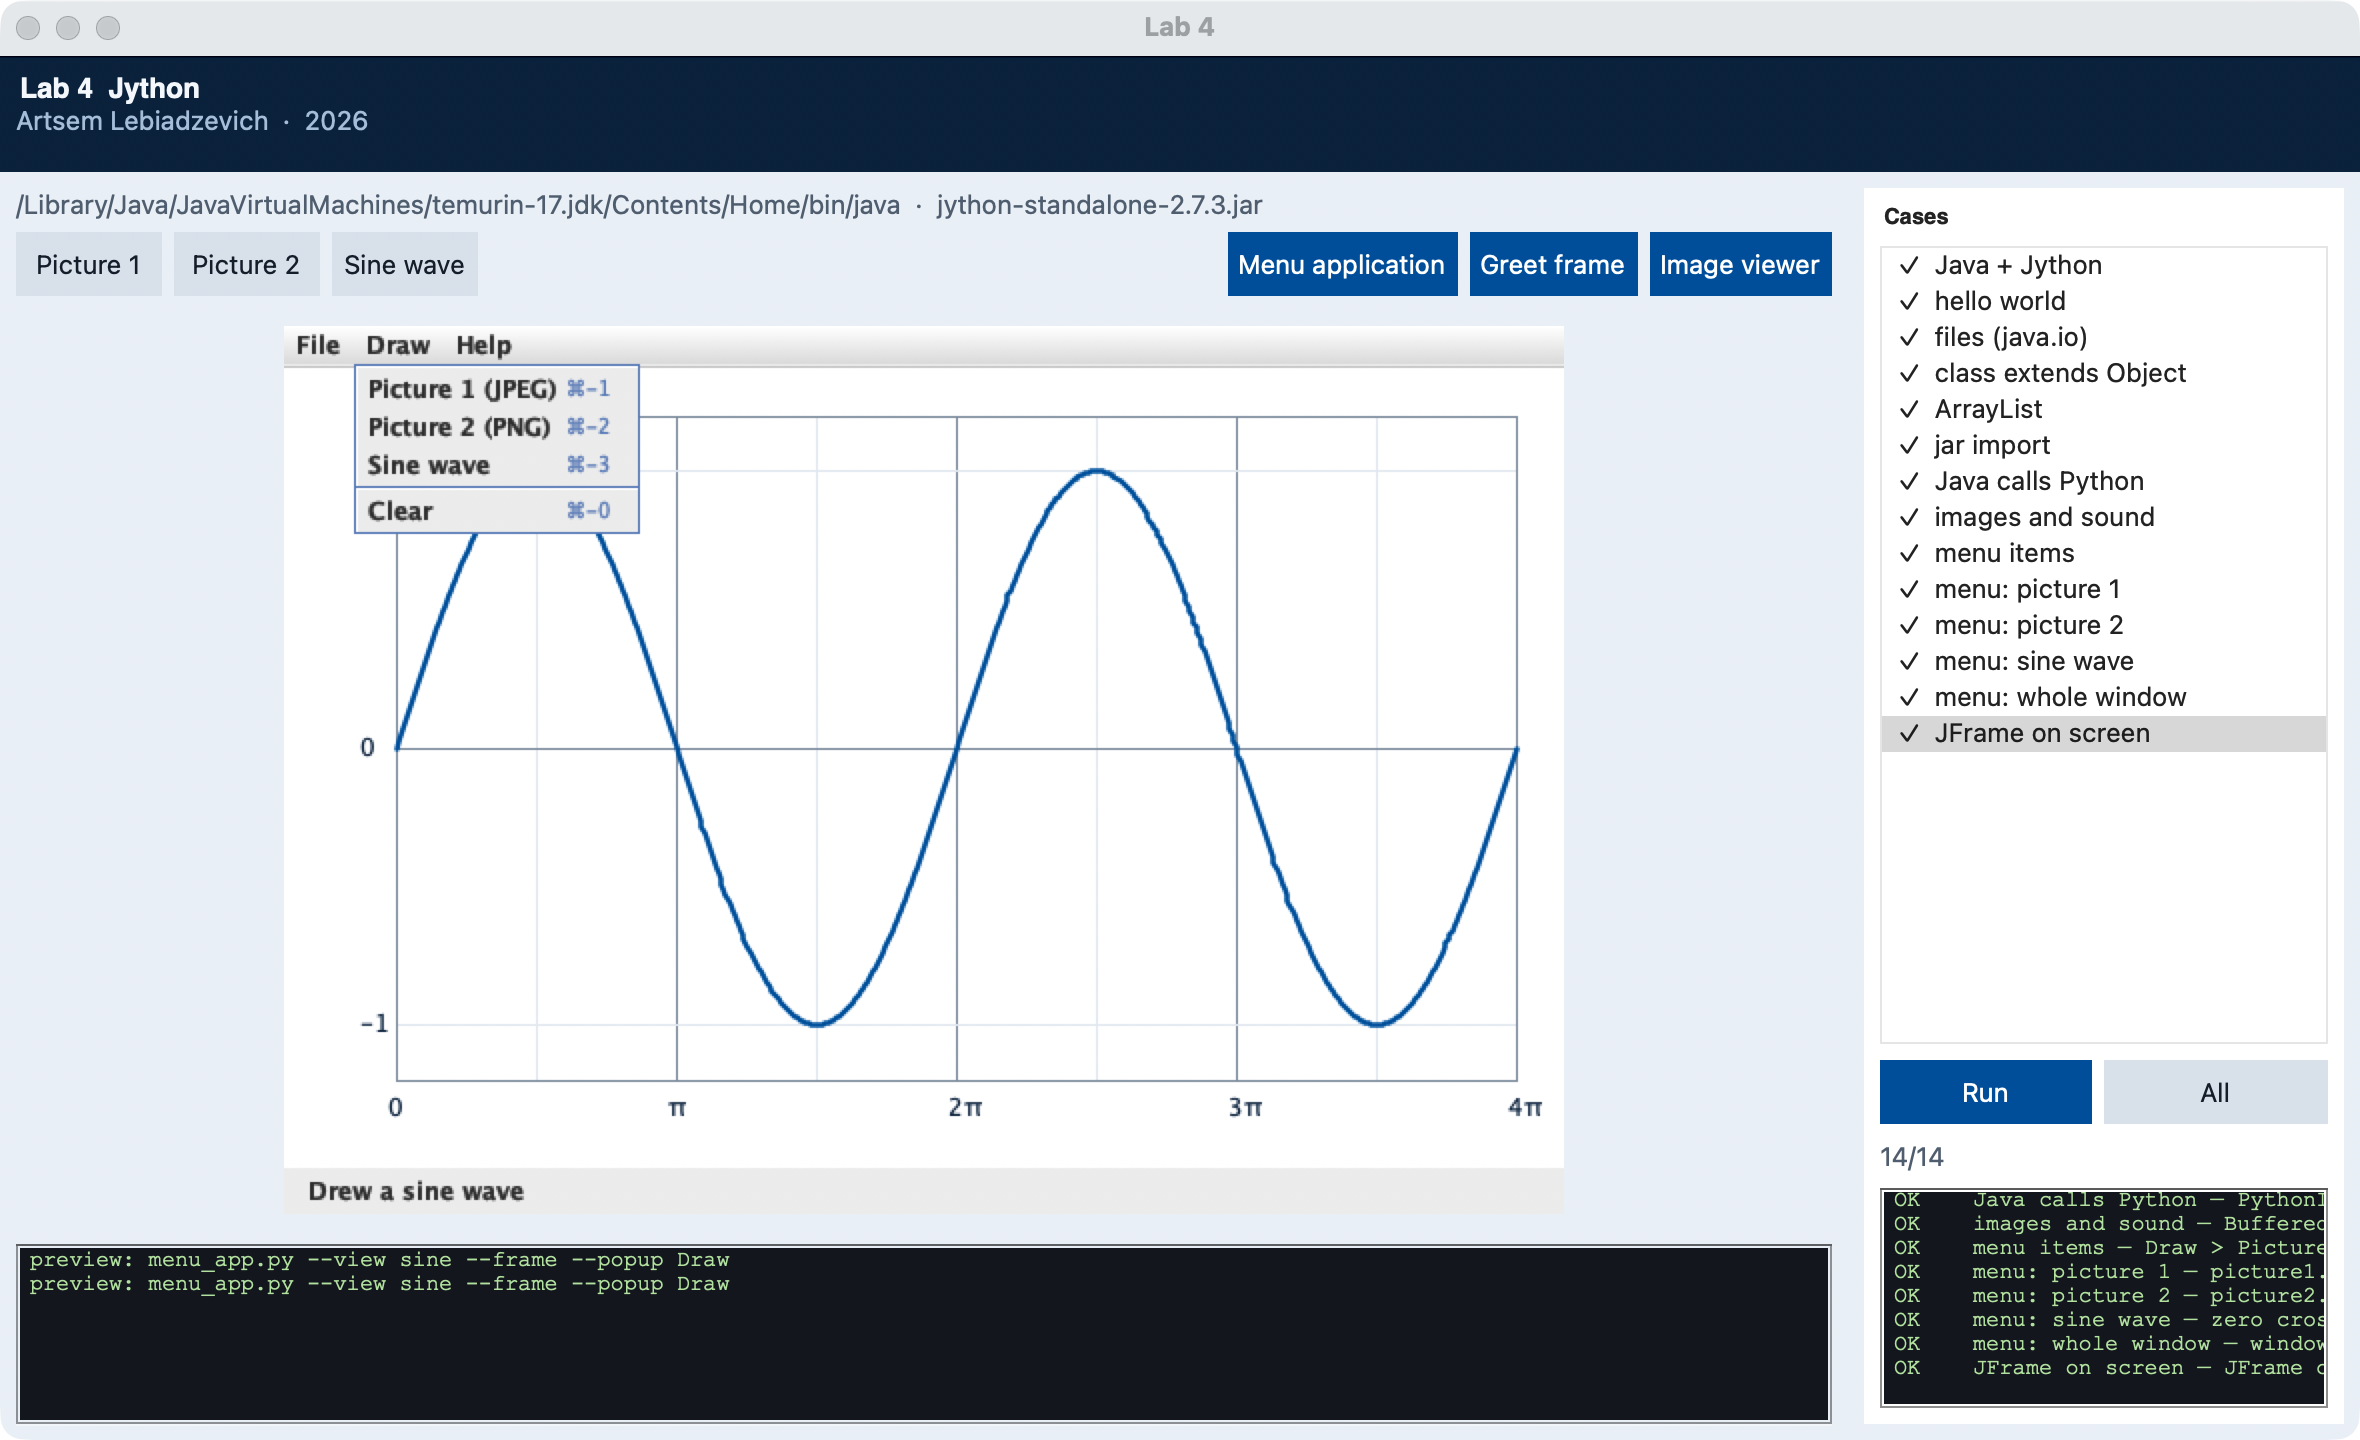
\includegraphics[width=0.95\textwidth]{../screenshots/lab4.png}
\caption{Окно лабораторной работы: снимок приложения и список проверок}
\label{fig:window}
\end{figure}

Содержимое окна приложения для каждого пункта меню показано на
рисунках~\ref{fig:p1}--\ref{fig:menu}.

\begin{figure}[H]
\centering
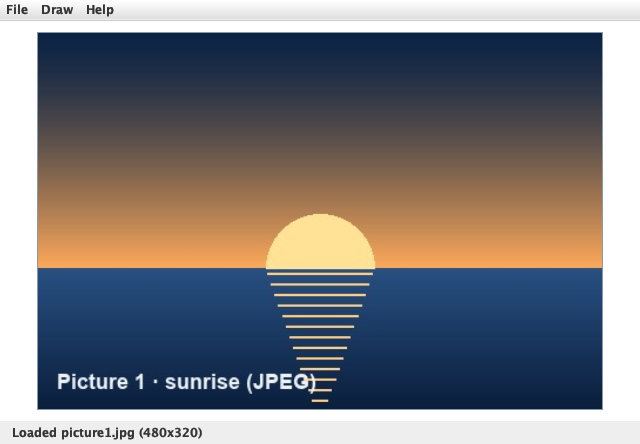
\includegraphics[width=0.8\textwidth]{../screenshots/lab4_picture1.png}
\caption{Draw $\rightarrow$ Picture 1: файл JPEG}
\label{fig:p1}
\end{figure}

\begin{figure}[H]
\centering
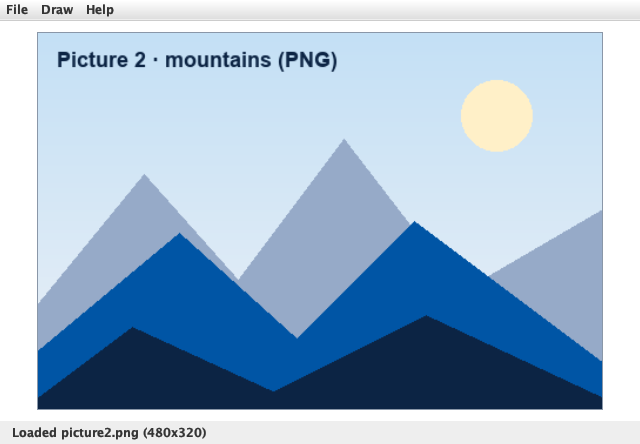
\includegraphics[width=0.8\textwidth]{../screenshots/lab4_picture2.png}
\caption{Draw $\rightarrow$ Picture 2: файл PNG}
\label{fig:p2}
\end{figure}

\begin{figure}[H]
\centering
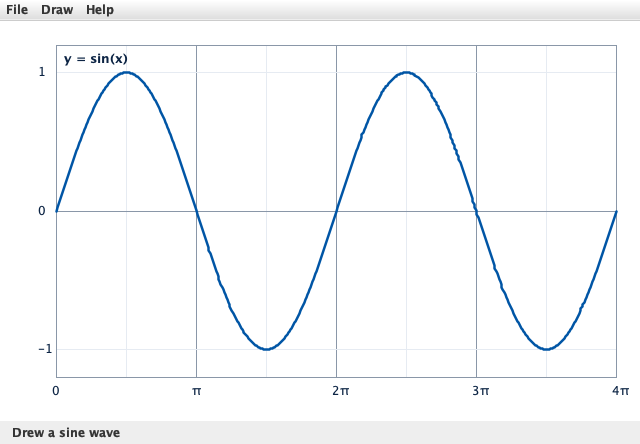
\includegraphics[width=0.8\textwidth]{../screenshots/lab4_sine.png}
\caption{Draw $\rightarrow$ Sine wave: $y=\sin x$ на отрезке $[0,4\pi]$}
\label{fig:sine}
\end{figure}

\begin{figure}[H]
\centering
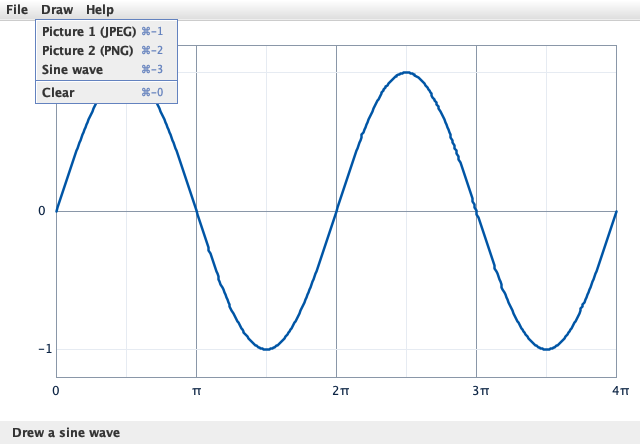
\includegraphics[width=0.8\textwidth]{../screenshots/lab4_menu.png}
\caption{Раскрытое меню Draw с сочетаниями клавиш}
\label{fig:menu}
\end{figure}

Команда \texttt{python main.py -{}-lab 4} выполняет сценарии без окна; вывод приведён в
листинге~\ref{lst:cli}. Результат проверяется по пикселям (таблица~\ref{tab:results}):
сравнение с исходным файлом, а не только отсутствие ошибки.

\lstinputlisting[style=plain, caption={Вывод программы}, label={lst:cli}]{listings/cli_output.txt}

\begin{table}[H]
\caption{Проверяемые сценарии}
\label{tab:results}
\centering
\small
\begin{tabularx}{\textwidth}{lL}
\toprule
Сценарий & Что проверяется \\
\midrule
environment & версии Java и Jython, время из Java близко к времени компьютера \\
hello world, files & вывод двумя способами; файл создан средствами \texttt{java.io},
содержимое прочитано из Python \\
class extends Object & экземпляр класса Python --- объект Java \\
ArrayList, jar import & коллекция Java в цикле Python; класс из jar-файла после
\texttt{sys.path.append} \\
Java calls Python & \texttt{PythonInterpreter}: \texttt{exec}, импорт модуля, \texttt{set} и
\texttt{get} \\
images and sound & в \texttt{BufferedImage} красный прямоугольник в нужной точке; JPEG
размером $480\times320$; формат WAV \\
menu items & нажатие четырёх пунктов меню меняет состояние холста \\
picture 1, picture 2 & холст совпадает с файлом, масштабированным в тот же прямоугольник
(ошибка меньше 1 из 255) \\
sine wave & кривая непрерывна, нули в точках $\pi,2\pi,3\pi$ ($\pm3$ пикселя), первый
максимум в $\pi/2$, амплитуда $1/1{,}2$ высоты \\
whole window & размер окна больше холста, раскрытое меню меняет снимок \\
JFrame on screen & настоящее окно открыто, \texttt{Greet} печатает имя, \texttt{Clear}
очищает поле \\
\bottomrule
\end{tabularx}
\end{table}

Автоматические тесты (\texttt{python -m unittest tests.test\_labs}) повторяют основные
проверки и пропускаются, если не найдены Java или jar-файл Jython. Все тесты проходят.

\section{Ответы на контрольные вопросы}

\textbf{1. Что такое Jython и как его запускают?} Реализация Python 2.7 для
виртуальной машины Java. Запуск: \texttt{java -jar jython-standalone-2.7.3.jar
script.py} либо установленным лаунчером \texttt{jython}.

\textbf{2. Как использовать классы Java в программе Jython?} Импортировать как
обычные имена (\texttt{from java.io import File}) и вызывать их методы. Исключения
Java перехватываются инструкцией \texttt{except}, от классов Java можно наследовать
(\texttt{class MyClass(Object)}), а коллекции Java допускают цикл \texttt{for} и
\texttt{len}.

\textbf{3. Как подключить классы из jar-файла?} Добавить файл в путь импорта
(\texttt{sys.path.append("x.jar")}) или указать \texttt{-classpath}, затем
\texttt{from com import MyClass}.

\textbf{4. Как вызвать Python из Java?} Добавить jar-файл Jython в путь классов и
использовать \texttt{PythonInterpreter}: \texttt{exec} выполняет код, \texttt{set} и
\texttt{get} передают значения.

\textbf{5. Объясните решение лабораторной работы.} Класс \texttt{Canvas} --- панель
Swing, метод \texttt{paintComponent} которой рисует либо масштабированную картинку, либо
оси и синусоиду. Пункты меню используют общий \texttt{ActionListener}, который по
команде пункта переключает холст. Меню и холст собраны в \texttt{JRootPane}, поэтому их
можно нарисовать в файл и проверить без экрана.

\sectioncenter{Заключение}

В ходе лабораторной работы изучено взаимодействие Java и Python через Jython.
Выполнены все примеры методических материалов и лекции: классы Java используются в
Python, класс Python наследует класс Java, jar-файл подключается к программе, а
программа на Java запускает код Python. Создано приложение с окном \texttt{JFrame},
меню которого загружает две разные картинки (JPEG и PNG) и рисует синусоиду на холсте.

Практический вывод: Jython делает классы Java обычными именами Python, но привязывает
программу к Python 2.7 и к версии JDK. Для JDK 17 импорты из методички потребовали
обходного пути (\texttt{sys.add\_package}). Размещение рисования в \texttt{JPanel}, а
меню --- в \texttt{JRootPane} позволило проверить графическое приложение по
пикселям, не открывая окна.

\sectioncenter{Список использованных источников}

\begin{enumerate}
\item Герман, О.~В. Jython: лекция и лабораторная работа по дисциплине <<Технологии
компонентного программирования>> / О.~В.~Герман. --- Минск: БГУИР, 2024.
\item Jython Documentation [Электронный ресурс]. --- Режим доступа:
\url{https://www.jython.org/}.
\item Pedroni, S. Jython Essentials / S.~Pedroni, N.~Rappin. --- Sebastopol:
O'Reilly, 2002. --- 296~p.
\item The Java Tutorials: Creating a GUI With Swing [Электронный ресурс]. --- Режим
доступа: \url{https://docs.oracle.com/javase/tutorial/uiswing/}.
\end{enumerate}

\end{document}
